\documentclass{article}
\usepackage{setspace,tikz,wrapfig}
\usepackage[text={6.5in,8.5in},centering]{geometry}
\geometry{verbose,a4paper,tmargin=2.4cm,bmargin=2.4cm,lmargin=2.4cm,rmargin=2.4cm}
\usepackage{graphicx,amsmath,cases,multirow,appendix,graphicx,xcolor}

\setlength\parindent{0pt}

\newcommand{\note}[1]{\colorbox{gray!30}{#1}}
\newcommand{\ind}{\-\hspace{1cm}}
\newcommand*\circled[1]{\tikz[baseline=(char.base)]{
            \node[shape=circle,draw,inner sep=2pt] (char) {#1};}}
\newenvironment{rcases}
  {\left.\begin{aligned}}
  {\end{aligned}\right\rbrace} 

\renewcommand\floatpagefraction{.9}
\renewcommand\topfraction{.9}
\renewcommand\bottomfraction{.9}           

\begin{document}

\noindent\makebox[\textwidth][c]{\Large\bfseries Lecture 11 -- 2-D Stability Analysis -- Competition Part 2}
\rule[0.5ex]{\linewidth}{1pt}
\textbf{Today:} 
\ind Formal stability analysis of two-species competition equilibria\\
\textbf{Next class} move on to Consumer-Resource \& nonlinear interactions.

\rule[0.5ex]{\linewidth}{1pt}

\textbf{Evaluate stability of equilibria} \\
Just as for 1 species model:\\
\ind Step \#1: Solve for $N^*$ steady state equilibria\\
\ind Step \#2: Find $f'$ and evaluate at $N^*$

Let's use non-dimensionalized version of the LV-competition model!\\
Let:
\begin{align*}
	u_1 = \frac{N_1}{K_1} \quad & \quad u_2 = \frac{N_2}{K_2} \quad  \quad \quad \quad \tau = r_1 t\\
	\rho = \frac{r_2}{r_1} \quad & \quad a_{12}=\alpha_{12}\frac{K_2}{K_1} \quad \quad a_{21}=\alpha_{21}\frac{K_1}{K_2} 
\end{align*}
\ind $u_i$ - \% of carrying capacity\\
\ind $\tau$ - `growth time'\\
\ind $\rho$ - relative growth rates\\
\ind $a_{ij}$ - relative resource requirements\\


New model becomes:
\begin{equation*}
	\frac{d u_1}{d\tau}=u_1(1-u_1 - a_{12}u_2) \quad \quad \frac{d u_2}{d\tau}=\rho u_2(1-u_2 - a_{21}u_1)
\end{equation*}

\note{$\Rightarrow$ Mathematica \emph{`Class10-LVcompetition-nonDim'}}
\vspace{0.5cm}

Isoclines:
\begin{equation*}
	u_1^*=\frac{1-u_2}{a_{21}} \quad \quad u_2^*=\frac{1-u_1}{a_{12}}
\end{equation*}

\
\textbf{Step \#1}: Solve for $u^*$ steady state equilibria
\begin{align*}
(u_1^*,u_2^*)& =
\begin{cases}
	 0 , & 0  \\
	0, & 1  \\
	1, & 0\\
	\frac{1-a_{12}}{1- a_{12} a_{21} }, & \frac{1-a_{21}}{1- a_{12} a_{21} } \quad \text{\note{multiply Mathematica output top by -1, then top and bottom by -1}}
\end{cases}
\end{align*}


\textbf{Step \#2:} Evaluate $f'(N^*)$ \\
\ind \ind \ind \ind ...but now in two dimensions:  $f_1'(N_1^*,N_2^*)$ and $f_2'(N_1^*,N_2^*)$\\

\begin{center}
	$\Rightarrow$ \textbf{Stability analysis in two dimensions} $\Leftarrow$\\
\end{center}

Perturbation to both $u_1^*$ and $u_2^*$ by amounts $x$ and $y$.
\begin{align*}
	u_1 & = u_1^* + x \quad \quad u_2  = u_2^* + y\\
	\Rightarrow \quad x & =u_1^* - u_1 \quad \quad y  = u_2^* - u_2
\end{align*}

\begin{center}
	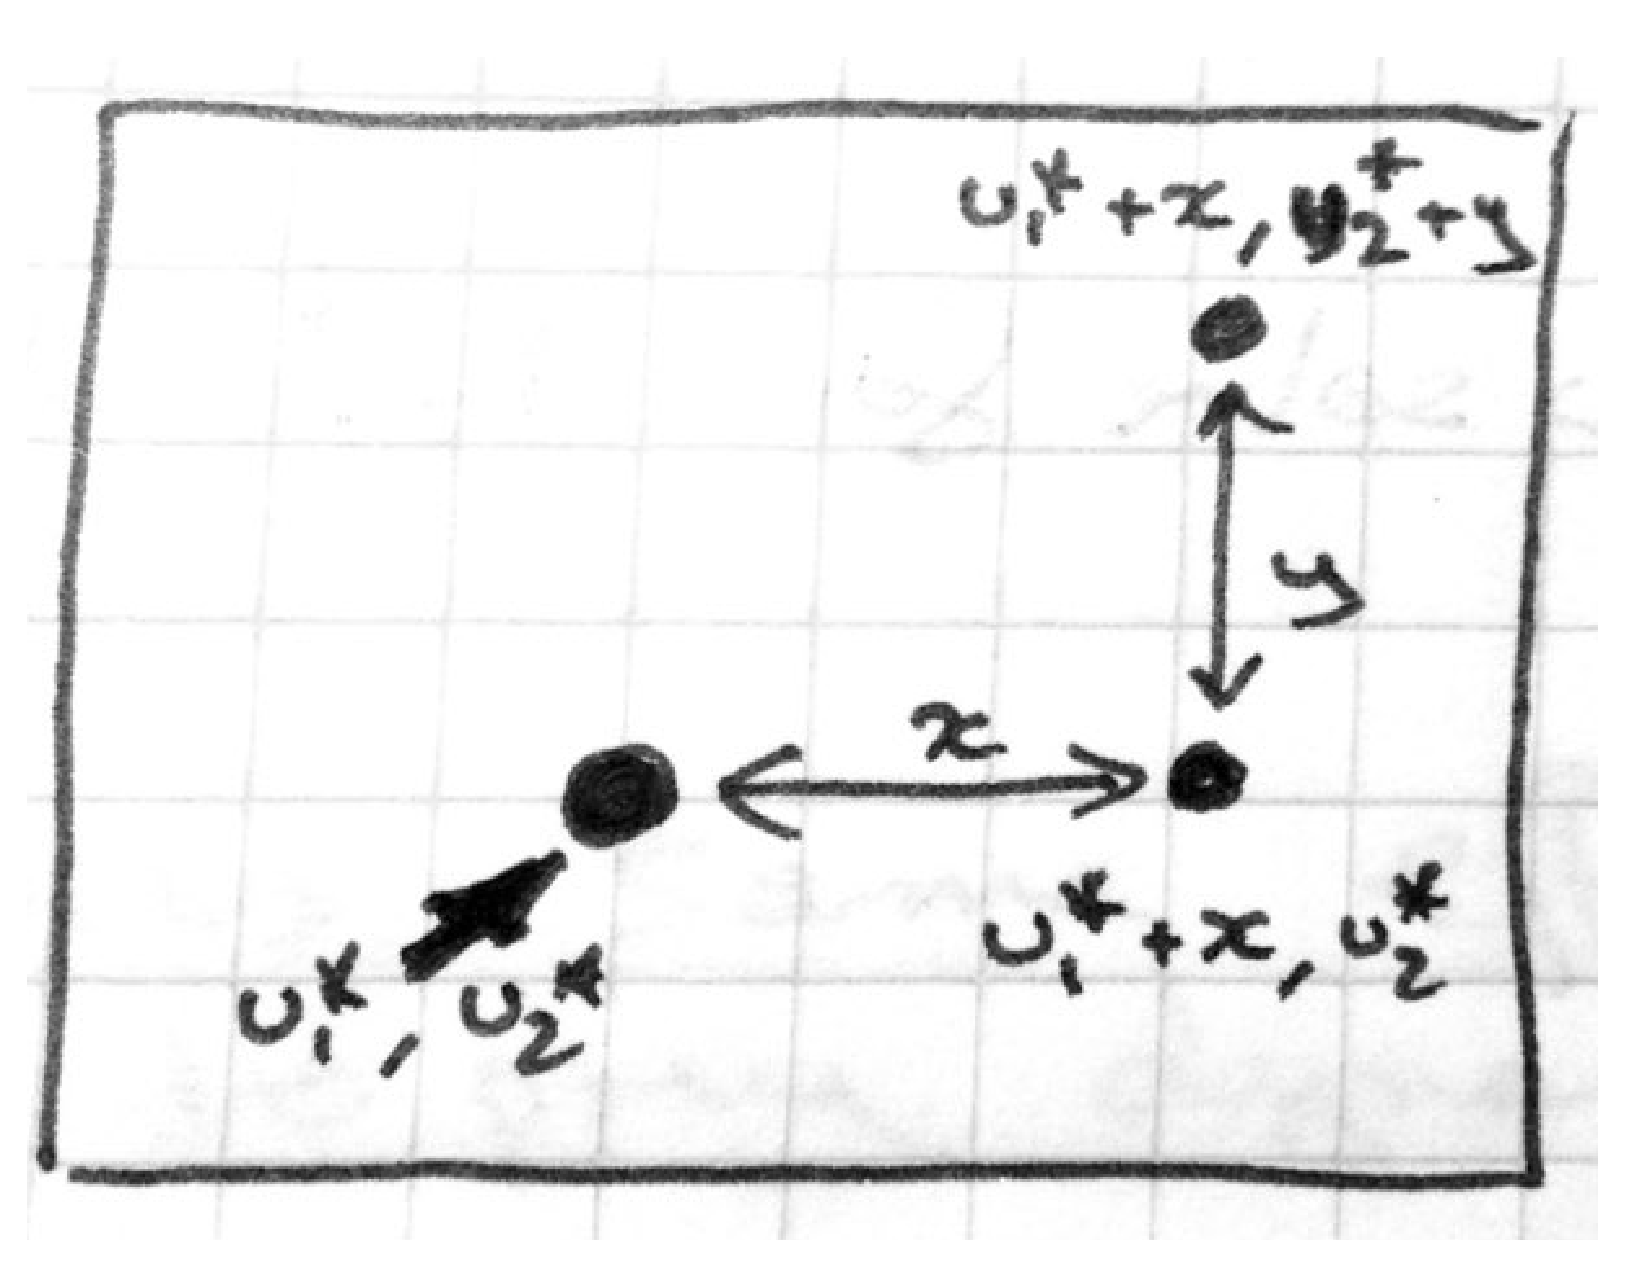
\includegraphics[width=6cm]{figs/2Dperturb.pdf}
\end{center}

Thus:
\begin{align*}
	&\frac{du_1}{d\tau}=\frac{d (u_1^* + x)}{d\tau}=f_1(u_1^*+x,u_2^*+y)\\
	\text{ and} &\\
	&\frac{du_2}{d\tau}=\frac{d (u_2^* + y)}{d\tau}=f_2(u_1^*+x,u_2^*+y)	
\end{align*}
Because $u_1^*$ and $u_2^*$ are constants w.r.t $\tau$...
\begin{align*}
	&\frac{dx}{d\tau} = \frac{du_1}{d\tau}\\
	\text{and}&\\
	&\frac{dy}{d\tau}= \frac{du_2}{d\tau}
\end{align*}

Recall that we approximated response of single-sp.~perturbation using a Taylor expansion:\\
\begin{equation*}
	f(N^*+n_t)\approx f(N^*)+f'(N^*) \cdot n_t + h.o.t.
\end{equation*}

Do same thing in two dimensions (note use of \emph{partial} derivatives):\\

To simplify syntax, let's denote $f_i(u_1^*,u_2^*) = f_i$\\
\ind (i.e. $f_i$ is implicitly evaluated at steady state abundances)
\begin{align*}
	f_1(u_1^* + x, u_2^* + y) = & f_1(u_1^*,u_2^*) + \frac{\partial f_1}{1! \phantom{.}\partial u_1} \cdot x + \frac{\partial^2 f_1}{2! \phantom{.} \partial u_1^2} \cdot x^2 + h.o.t. + \dots \\
	&\quad \quad \quad \quad \dots  + \frac{\partial f_1}{1!\phantom{.} \partial u_2} \cdot y + \frac{\partial^2 f_1}{2!\phantom{.} \partial u_2^2} \cdot y^2 +  h.o.t.\\
	 \approx & f_1(u_1^*, u_2^*) + \left. \frac{\partial f_1}{\partial u_1}\right|_{u_1^*, u_2^*} \cdot x + \left. \frac{\partial f_1}{\partial u_2}\right|_{u_1^*, u_2^*} \cdot y
\end{align*}
Since at steady-state (by definition)..
\begin{equation*}
	f_1(u_1^*,u_2^*)=0
\end{equation*}
...we can simplify further to:
\begin{equation*}
	f_1(u_1^* + x, u_2^* + y)\approx \underbrace{\left. \frac{\partial f_1}{\partial u_1}\right|_{u_1^*, u_2^*}}_{A_{11}} \cdot x + \underbrace{\left. \frac{\partial f_1}{\partial u_2}\right|_{u_1^*, u_2^*}}_{A_{12}} \cdot y
\end{equation*}

Similarly
\begin{equation*}
	f_2(u_1^* + x, u_2^* + y)\approx \underbrace{\left. \frac{\partial f_2}{\partial u_1}\right|_{u_1^*, u_2^*}}_{A_{21}} \cdot x + \underbrace{\left. \frac{\partial f_2}{\partial u_2}\right|_{u_1^*, u_2^*}}_{A_{22}} \cdot y
\end{equation*}

Organize these elements into a \emph{\textbf{Jacobian matrix}}:
\begin{equation*}
\mathbf{A}=
	\begin{bmatrix}
	A_{11} & A_{12}\\
	A_{21} & A_{22}
	\end{bmatrix}.
\end{equation*}

Jacobian contains the partial derivatives of each $i^{th}$ variable's function $f_i$ w.r.t $j$.\\

\textbf{A} is referred to as the \emph{\textbf{Community matrix}} when $f_i$'s reflect population growth rates (i.e. $f_i=\tfrac{dN_i}{dt}$).\\

\emph{Interpretation of elements:}\\
\ind How a small perturbation to $j$ affects the population growth rate of $i$\\
\ind \ind \ind \ind \ind \ind  \ind \ind \ind \emph{with other species held constant}\\

\rule[0.5ex]{\linewidth}{1pt}

\pagebreak

The Jacobian's eigenvalues provide insight into the stability of the steady state(s).\\
We will return to this in more detail next time.\\
\ind For now note that eigenvalues can have both `Real' and `Imaginary' parts...

\begin{center}
	\begin{tabular}{ll}
		\hline
		\textbf{Eigenvalues ($\lambda_i$)} & \textbf{Interpretation} \\ 
		\hline
		$Re(\lambda_i)< 0$  for all $i$& Stable node (point attractor)\\ 
		$Re(\lambda_i)< 0$ for some $i$ & Saddle node (repellor-attractor) \\ 
		$Re(\lambda_i)> 0$ for all $i$ & Unstable node (repellor)\\ 
		$Re(\lambda_i) = 0$ for all $i$ & Neutrally stable \\ 
		\hline
		$Im(\lambda_i) = 0$ for all $i$ & No oscillations \\ 
		$Im(\lambda_i) \neq 0$ for some $i$  & Oscillations \\ 
		\hline
	\end{tabular} 
\end{center}

\rule[0.5ex]{\linewidth}{1pt}

\textbf{Evaluate eigenvalues of LV-competition equilibria}\\
\ind \note{$\Rightarrow$ Mathematica \emph{`Class11-LVcompetition-nonDim'}}\\

(Scenario 1) When intra- is stronger than inter-specific competition for both species\\
 \ind (i.e.~$a_{ij} < a_{ii} = 1$ for both)
\begin{center}
	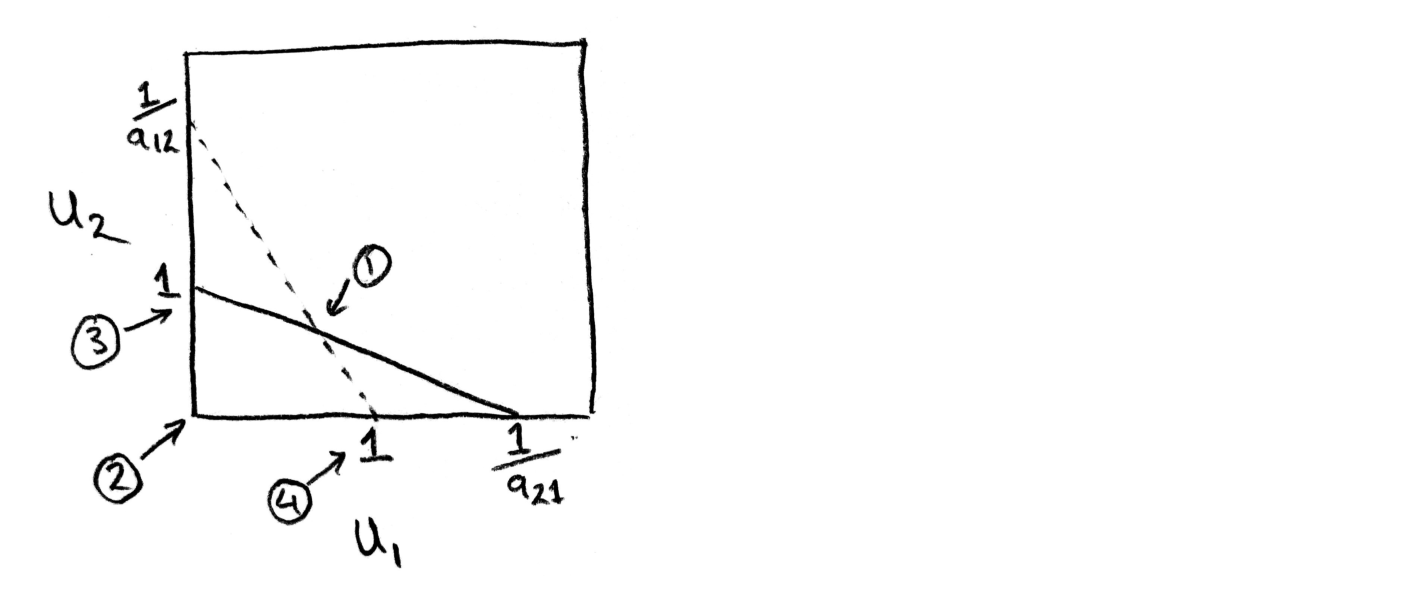
\includegraphics[width=5.2cm]{figs/LVcomp-Case1.pdf}
\end{center}
\ind \circled{1} Both $\lambda's <0 \Rightarrow$ Stable coexistence\\
\ind \circled{2} Both $\lambda's > 0 \Rightarrow$ Unstable\\
\ind \circled{3} $\lambda_1>0$ \& $\lambda_2 <0 \Rightarrow$ unstable (attractor-repellor)\\
\ind \circled{4} $\lambda_1<0$ \& $\lambda_2 >0 \Rightarrow$ unstable (attractor-repellor) \\
\ind $\implies$
 \circled{3} and \circled{4} are mutually invasible\\

(Scenario 2) When inter- is stronger than intra-specific competition for both species\\
\ind (i.e.~$a_{ij} > a_{ii} = 1$ for both)
\begin{center}
	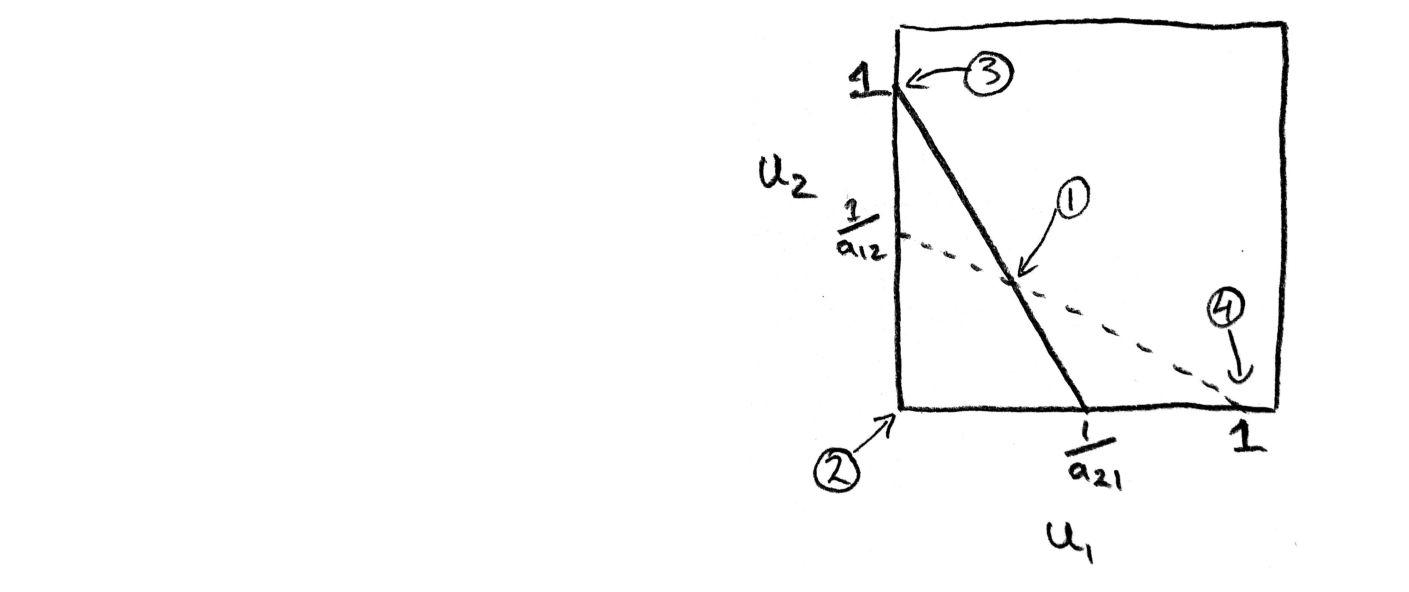
\includegraphics[width=5.2cm]{figs/LVcomp-Case2.pdf}
\end{center}
\ind \circled{1} $\lambda_1<0$ \& $\lambda_2 > 0 \Rightarrow$ unstable (attractor-repellor)\\
\ind \circled{2} Both $\lambda's > 0 \Rightarrow$ Unstable\\
\ind \circled{3} \circled{4} Both $\lambda's < 0 \Rightarrow$ Stable\\

\ind $\implies$
\circled{3} and \circled{4} are Alternative Stable States


\rule[0.5ex]{\linewidth}{1pt}
\rule[0.5ex]{\linewidth}{1pt}


\end{document}